\documentclass[12pt,x11names,a4paper]{article}
\input{preamble}


\newgeometry{margin=2cm}

\pagestyle{fancy}
\fancyhf{}

\rhead{Nørre Gymnasium\\3.c
}
\cfoot{Side \thepage \hspace{1pt} af \pageref{LastPage}}

%Husk at rette modul og dato!
\lhead{Aflevering 8\\ Matematik A
}
\chead{25. januar 2024
}

\begin{document}

%
\includepdf[pages=-]{Forsider/aarsprove_1v.pdf}
\savegeometry{art}

\begin{titlepage}
\newgeometry{margin=0pt}

\begin{minipage}{0.27\textwidth}

\begin{tikzpicture}[overlay]
\fill[top color = NorregGroen!40, bottom color = NorregGroen] (6,10) rectangle (-10,-30);
\end{tikzpicture}
\end{minipage}
\begin{minipage}{0.73\textwidth}
\begin{center}
\phantom{h} \vspace{1cm}\\
\hspace{4cm}

\includegraphics[scale = 1]{Billeder/Norreg.png} \\
\phantom{h} \vspace{5cm}\\
\rule{0.7\textwidth}{0.3mm}\\
\phantom{h}\\
{\fontsize{50}{60}\selectfont Matematik-\\aflevering}\\
\phantom{h}\\
\rule{0.7\textwidth}{0.3mm}\\
\Large 2024\\
\Large 3.c MA

\end{center}
\end{minipage}
\end{titlepage}
\loadgeometry{art}

%Udfyld afsnit herunder og lav til egen Latex-fil

%Kopier følgende til overskrift:

%\begin{center}
%\Huge
%Aflevering 1
%\end{center}
%\section*{Opgave 1}
%\stepcounter{section}
\begin{center}
%Opgavesætter er delt i to dele:\\
%Delprøve 1 kun med den centralt udmeldte formelsamling.\\
%Delprøve 2 med alle hjælpemidler.
\end{center}

\section*{Krav til formidling af din besvarelse}

Ved bedømmelse af helhedsindtrykket af besvarelsen af de enkelte opgaver lægges særlig vægt på følgende fire punkter:
\begin{itemize}
\item[$\cdot$] \textbf{Redegørelse og dokumentation for metode} \\
Besvarelsen skal indeholde en redegørelse for den anvendte løsningsstragegi med dokumentation i form af et passende antal mellemregninger \textit{eller} matematiske forklaringer på metoden, når et matematisk værktøjsprogram anvendes.
\item[$\cdot$] \textbf{Figurer, grafer og andre illustrationer} \\
Besvarelsen skal indeholde hensigtsmæssig brug af figurer, grafer og andre illustrationer, og der skal være tydelige henvisninger til brug af disse i den forklarende tekst.
\item[$\cdot$] \textbf{Notation og layout}\\
Besvarelsen skal i overensstemmelse med god matematisk skik opstilles med hensigtsmæssig brug af symbolsprog, og med en redegørelse for den matematiske notation, der indføres og anvendes, og som ikke kan henføres stil standardviden.
\item[$\cdot$] \textbf{Formidling og forklaring}\\
Besvarelsen af rene matematikopgaver skal indeholde en angivelse af givne oplysninger og korte forklaringer knyttet til den anvendte løsningsstrategi beskrevet med brug af almindelig matematisk notation. 

Besvarelsen af opgaver, der omhandler matematiske modeller, skal indeholde en kort præsentation af modellens kontekst, herunder betydning af modellens parametre. De enkelte delspørgsmål skal afsluttes med en præcis konklusion præsenteret i et klart sprog i relation til konteksten.
\end{itemize}

\newpage

\section*{Med hjælpemidler}
\begin{opgavetekst}{Opgave 1}
	\begin{center}
		\includegraphics[width=0.6\textwidth]{Billeder/chips}
	\end{center}
	Vægten af en pose chips (i gram) er approksimativt normalfordelt med den normalfordelte 
	stokastiske variabel
	\begin{align*}
		X \sim \textnormal{N}(120,2).
	\end{align*}
\end{opgavetekst}
\begin{delopgave}{}{1}
	Afgør, om en pose på 113 gram er et exceptionelt udfald.
\end{delopgave}
\begin{delopgave}{}{2}
	Forklar, hvad integralet 
	\begin{align*}
		\int_{120}^{123}\frac{1}{\sqrt{2\pi}2}e^{-\frac{1}{2}\left(\frac{x-120}{2}\right)^2}dx
		\approx 0.433
	\end{align*}
	siger om chipsposerne.
\end{delopgave}


\begin{opgavetekst}{Opgave 2}
	Fordelingsfunktionerne $F_X$ og $F_Y$ for to stokastiske variable
	\begin{align*}
		&X \sim \textnormal{N}(\mu_X,2)\\
		&Y \sim \textnormal{N}(\mu_Y,3)
	\end{align*}
	er givet på Figur \ref{fig:fordeling}.
	\begin{figure}[H]
		\centering
		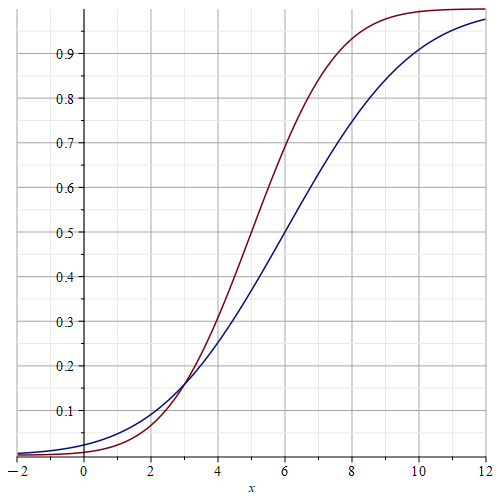
\includegraphics[width=0.6\textwidth]{Billeder/fordelinger}
		\caption{Graferne for fordelingsfunktionerne for $X$ og $Y$}
		\label{fig:fordeling}
	\end{figure}
	\phantom{h}
\end{opgavetekst}
\begin{delopgave}{}{1}
	Afgør hvilken af graferne der tilsvarer $F_X$ og hvilken, der tilsvarer $F_Y$.
\end{delopgave}
\begin{delopgave}{}{2}
	Bestem $\mu_X$ og $\mu_Y$.
\end{delopgave}
\begin{delopgave}{}{3}
	Bestem sandsynligheden $P(4<Y<8)$.
\end{delopgave}


\begin{opgavetekst}{Opgave 3}
	\begin{center}
		\includegraphics[width=0.6\textwidth]{Billeder/helpizza}
	\end{center}
	Hos en producent af pizzaer har man lavet en stikprøve på 100 pizzaer. Man har målt deres
	diameter, og antager at denne er normalfordelt. Resultatet af stikprøven kan findes 
	\href{https://github.com/ChristianJLex/TeachingNotes/raw/master/2023-2024/Data og lign/Pizzaradius.xlsx}{\color{blue!60} her.}
\end{opgavetekst}
\begin{delopgave}{}{1}
	Argumentér for at pizzaernes diameter er tilnærmelsesvist normalfordelte, og bestem den 
	estimerede middelværdi og estimerede spredning for den normalfordelte stokastiske variabel
	$X$, der beskriver diameteren.
\end{delopgave}
\begin{delopgave}{}{2}
	Bestem intervallet for de normale udfald for diameteren af pizzaerne.
\end{delopgave}
\begin{delopgave}{}{3}
	Bestem $z$-værdien for udfaldet 33cm og brug denne til at afgøre, om 33 er et exceptionelt
	udfald.
\end{delopgave}
\begin{meretekst}
	Producenten af pizzaer har en forventning om, at under 1$\%$ af deres pizzaer har en radius 	på under 29cm.
\end{meretekst}
\begin{delopgave}{}{4}
	Brug $X$ til at afgøre, om producenten opfylder sit ønske.
\end{delopgave}
\begin{meretekst}
	Producenten kan ikke ændre på spredningen af deres pizzaers diameter; de kan kun ændre på 
	middelværdien ved at tilføje lidt mere eller lidt mindre dej til hver pizza.
\end{meretekst}
\begin{delopgave}{}{5}
	\textbf{Ekstraopgave:} Bestem hvad middelværdien for $X$ skal være, hvis producenten skal
	opfylde sit ønske om, at kun 1$\%$ af pizzaerne har en diameter på under 29cm.
\end{delopgave}

\end{document}



